\documentclass[12pt,letterpaper]{article}

% just for the example
\usepackage{lipsum}
% Set margins to 1.5in
\usepackage[margin=1.5in]{geometry}
\usepackage[toc,page]{appendix}

% for graphics
\usepackage{graphicx}
\graphicspath{{./figures/m3/}}

% for crimson text
\usepackage{crimson}
\usepackage[T1]{fontenc}
\usepackage{url}

% setup parameter indentation
\setlength{\parindent}{0pt}
\setlength{\parskip}{6pt}

% for 1.15 spacing between text
\renewcommand{\baselinestretch}{1.15}

% For defining spacing between headers
\usepackage{titlesec}
% Level 1
\titleformat{\section}
  {\normalfont\fontsize{18}{0}\bfseries}{\thesection}{1em}{}
% Level 2
\titleformat{\subsection}
  {\normalfont\fontsize{14}{0}\bfseries}{\thesection}{1em}{}
% Level 3
\titleformat{\subsubsection}
  {\normalfont\fontsize{12}{0}\bfseries}{\thesection}{1em}{}
% Level 4
\titleformat{\paragraph}
  {\normalfont\fontsize{12}{0}\bfseries\itshape}{\theparagraph}{1em}{}
% Level 5
\titleformat{\subparagraph}
  {\normalfont\fontsize{12}{0}\itshape}{\theparagraph}{1em}{}
% Level 6
\makeatletter
\newcounter{subsubparagraph}[subparagraph]
\renewcommand\thesubsubparagraph{%
  \thesubparagraph.\@arabic\c@subsubparagraph}
\newcommand\subsubparagraph{%
  \@startsection{subsubparagraph}    % counter
    {6}                              % level
    {\parindent}                     % indent
    {12pt} % beforeskip
    {6pt}                           % afterskip
    {\normalfont\fontsize{12}{0}}}
\newcommand\l@subsubparagraph{\@dottedtocline{6}{10em}{5em}}
\newcommand{\subsubparagraphmark}[1]{}
\makeatother
\titlespacing*{\section}{0pt}{12pt}{6pt}
\titlespacing*{\subsection}{0pt}{12pt}{6pt}
\titlespacing*{\subsubsection}{0pt}{12pt}{6pt}
\titlespacing*{\paragraph}{0pt}{12pt}{6pt}
\titlespacing*{\subparagraph}{0pt}{12pt}{6pt}
\titlespacing*{\subsubparagraph}{0pt}{12pt}{6pt}

% Set caption to correct size and location
\usepackage[tableposition=top, figureposition=bottom, font=footnotesize, labelfont=bf]{caption}

% set page number location
\usepackage{fancyhdr}
\fancyhf{} % clear all header and footers
\renewcommand{\headrulewidth}{0pt} % remove the header rule
\rhead{\thepage}
\pagestyle{fancy}

% Overwrite Title
\makeatletter
\renewcommand{\maketitle}{\bgroup
   \begin{center}
   \textbf{{\fontsize{18pt}{20}\selectfont \@title}}\\
   \vspace{10pt}
   {\fontsize{12pt}{0}\selectfont \@author} 
   \end{center}
}
\makeatother

% Used for Tables and Figures
\usepackage{float}

% For using lists
\usepackage{enumitem}

% For using APA Citation format
\usepackage{apacite}

% Custom Quote
\newenvironment{myquote}[1]%
  {\list{}{\leftmargin=#1\rightmargin=#1}\item[]}%
  {\endlist}
  
% Create Abstract 
\renewenvironment{abstract}
{\vspace*{-.5in}\fontsize{12pt}{12}\begin{myquote}{.5in}
\noindent \par{\bfseries \abstractname.}}
{\medskip\noindent
\end{myquote}
}

\begin{document}

% Set Title, Author, and email
\title{Assignment M5}
\author{Snejana Shegheva \\ sshegheva3@gatech.edu}

\maketitle
\thispagestyle{fancy}

\begin{abstract}
Mapping data from one form to another for its ease-of-use is at the core of the \textit{Extract, Transform and Load} process. In this project, we evaluate various prototypes for an internal interface of a \textit{transform} task that prepares the data for use in a personalized recommendation system powered by Artificial Intelligence engines. The task involves altering the form of the received data with a purpose to extract relevant features in the form that is more advantageous for subsequent tasks. Our main goal is to assess all the weak areas of the suggested alternative models via early feedback collection from users who perform the task frequently and therefore have a good understanding of the task at hand.  
\end{abstract}

\section*{Qualitative Evaluation}
\subsubsection*{Think-aloud for Verbal Prototype}
\textit{Appendix} A contain verbal prototype that discusses a possible interface where a user is given a recommendation for which transformation function(s) is most compatible with the observed variable. The interface target both, novices who need to explore the system, and experts who aim to perform their tasks more efficiently.

\textbf{Evaluation Results}

The evaluation span across two sessions in the same day with the same participant. The first part took place in a casual setting of a short walk where I, as a "designer", engaged with the Product Manager in a conversation about the alternative design for the data transformation task. At the beginning of our conversation, I have set up the expectations for what I would like to get out of the discussion. The chosen participant has significant experience with the task at hand that contributed to a \textbf{productive session} given that the prototype was delivered verbally.

The second part of the evaluation happened a few hours later in the office setting. We choose to follow up on the remaining set of questions from the discussions that took place earlier. The participant expressed their feedback by sketching their thoughts on the piece of paper and elaborating on several analogies drawn from different tools and fields. Overall, the evaluation exceeded my expectations as it impacted how I was thinking about the design originally. 

\textbf{Reporting on the Results of the Think-Aloud Study}
To get started with the evaluation I described the idea to the user so they can imagine their workflow within the new interface. After they confirmed the understanding of new direction, I asked them to perform a specific transformation task while thinking aloud through the steps. \textit{Appendix B} contains the set of questions asked in the two sessions. As the questions were focused mostly on the actual use cases, for the simple examples (one-to-one transformations) the participant did not have a difficult time \textit{thinking-aloud} about the steps required to accomplish the task in the new interface. 

The user's thought process across all cases can be summarized with the following steps:

\begin{itemize}
    \item Find the input variable from a drop down list
    \item See the list of recommendations somewhere on the page
    \item Start from the top recommendation and evaluate its applicability to the case
    \item If it solves the case, then apply the recommendation and move on to the next variable
    \item If the recommendation is not applicable, go to the next recommendation in the list until the desired recommendation is found
\end{itemize}

The participant struggled with the use cases than required many-to-one or one-to-many transformations. I was asked to further elaborate on how the interface would support that. After additional guidance, the user was able to \textit{think} through the task, although they invoked imaginary steps not mentioned in the interface. Eventually, the conversation has shifted to how the user would prefer to accomplish the variations of the tasks by describing an alternative approach. As a result of the shift, questions 4 and 5 were on general satisfiability and learnability were not addressed directly, although I was able to infer them from the feedback that followed. Overall, the goal of the study was accomplished - the user has identified the usefulness and the limitation of the new interaction, and suggested ways to improve it.  

\textbf{Feedback from the Participant}

Although the user liked the idea of a \textit{recommended} transformations, they were not convinced that this would increase the efficiency of the task. The main take-away was that the recommendation should be focused on the \textit{outcome} instead of the \textit{function}. This is akin to flipping the problem in its head by starting from possible final results and walking backwards by narrowing down the steps to achieve the desired outcome. 

For example, if we have an unstructured field that contains \textit{dates}, recommending a transformation such as \textit{DateFinder} might be useful, however it does not communicate the result. If, instead, the interface suggests a few \textit{patterns} for what kinds dates \textit{can be} found in the text, then the user is able to make more informed decision on what type of transformations they wish to apply. The participant brought up a few analogies, such as Microsoft Excel's functionality for date transformation, and Spacy's Entity Recognition service. Figure~\ref{fig::1} demonstrates an example for using Spacy\footnote{https://spacy.io/ - Industrial-Strength
Natural Language Processing tool} tool for similar tasks of  pattern recognition. The user emphasized the \textit{intuitiveness} of  Spacy's interface.

\begin{figure}[h]
\centering
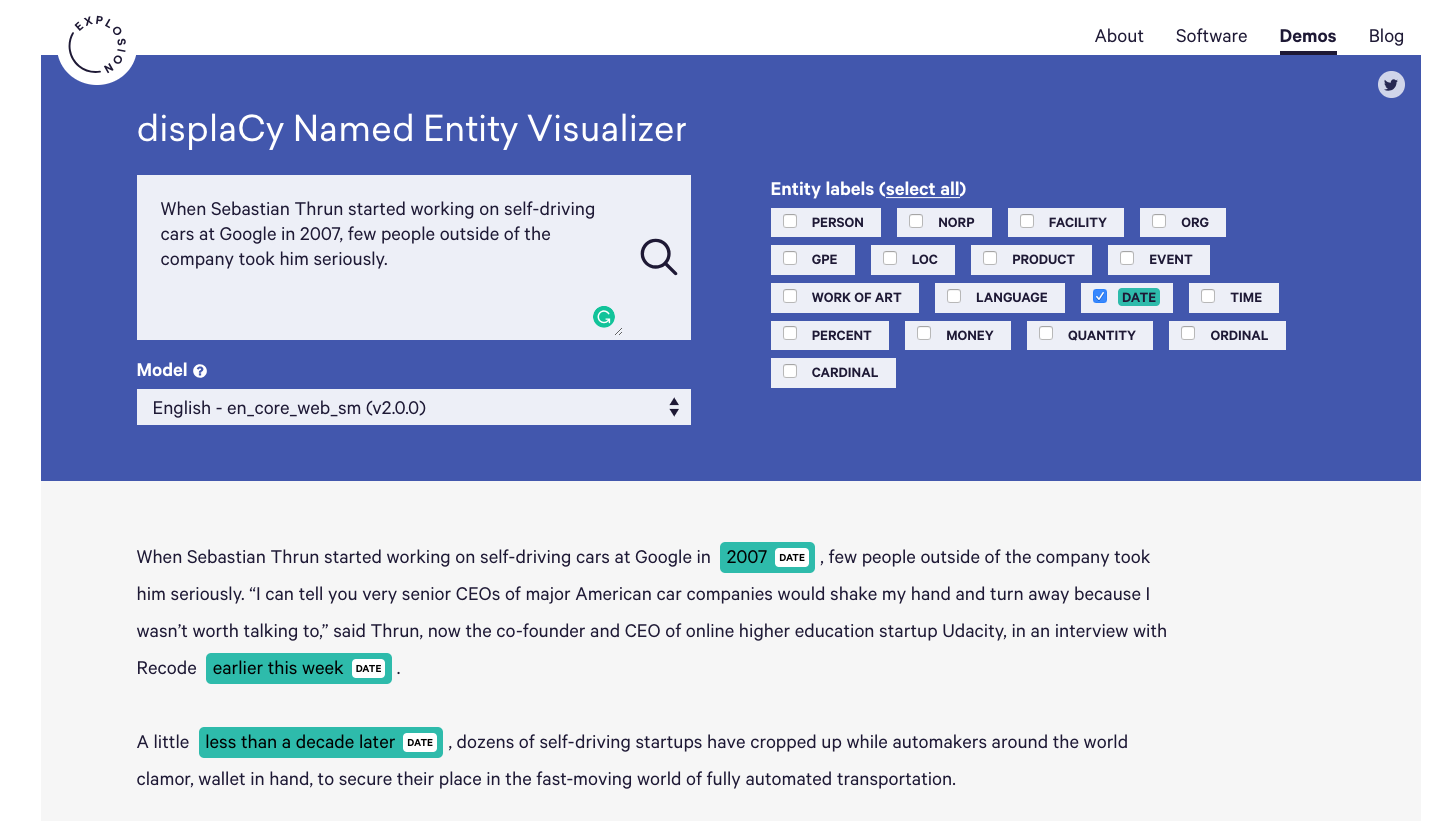
\includegraphics[scale=.3]{figures/m3/spacy_date_finder.png}
\caption{Example for pattern recognition for dates from DisplaCy Named Entity Visualizer (https://explosion.ai/demos/displacy-ent)}
\label{fig::1}
\end{figure}

The aspect of the feedback that surprised me the most that the user \textit{did not} seek solutions that would increase the speed of their task processing, or efficiency for finding the transformations. Based on my interpretation of their feedback, the user wanted an interface that would get them \textit{closer} to the data. Their ideal interaction seems to be \textit{discovering} the data, and a \textit{transformation} task is a way to extract specific elements from the text, and \textit{remember} those rules for subsequent streams of the same data.  

\textbf{Impact on the Prototype Design}
Based on the evaluation plan I need to re-iterate on the design cycle by brainstorming possible approaches for how to include \textit{previews} for possible \textit{outcomes} of transformations. 

\section*{Predictive Evaluation}

We are going to perform a \textbf{Cognitive Walkthrough} on the prototype shown in \textit{Appendix D}. The wireframes guide the user through the transformation task by keeping the sample of the data visible at all times. 

For the Cognitive Walkthrough, we identified the sequence of actions along with the series of questions that helps us evaluate the prototype.

\begin{itemize}
    \item \textbf{Step 1: Select a variable for transformation}
    \begin{itemize}
        \item Does the user understand what does it mean for a variable to be selected?
        \begin{itemize}
            \item Yes. By \textit{highlighting} the selected column, the interface is \textit{consistent} with other tools which means that user does not need an additional effort to learn the new interface. 
        \end{itemize}
        \item Can the user \textit{see} how the selection is accomplished? Is it visible on the screen or it requires filtering and contextual menus?
        \begin{itemize}
            \item No. The interface relies on the user having a good \textit{mental model} for how something can be selected. There are no visible menus or buttons for the selection step.  
        \end{itemize}
        \item Is the source variable clearly labeled?
            \begin{itemize}
                \item No. The header row contains all variable names available for the transformation, however, there is no label that marks the type of the variable. Users that deal with data on regular basis, would have no problem identifying the variables without labels, as it is \textit{consistent} with other data analysis tools.    
        \end{itemize}
        \item If the user is unable to select a variable, and the feedback is given to the user, can they understand and apply the feedback? 
        \begin{itemize}
                \item Yes. As the user hovers over the variable, the mouse cursor changes from an arrow to a pointer, therefore providing an \textit{affordance} that suggests how the user should interact with the displayed table of data.
        \end{itemize}
    \end{itemize}
    \item \textbf{Step 2: Apply the desired transformation function}
    \begin{itemize}
        \item Does the user have a correct conceptual model for that it means to change/transform the variable?
        \begin{itemize}
                \item Yes. When the user selects a variable, a contextual menu appears that suggests an operation for either creating a new variable based on the selected one, or edit the existing variable.
        \end{itemize}
        \item Can the user see the list of available transformation functions?
        \begin{itemize}
                \item Yes. When the user selects an operation, there are presented with a list of transformations, and a labeled action to choose a transformation. 
        \end{itemize}
        \item Do the functions' names reflect the clear operation?
        \begin{itemize}
                \item Yes. The names of the transformation demonstrate obvious \textit{signifiers} for the functions they perform. For example, if the user selected a textual variable and a transformation \textit{Remove Punctuation}, the user would have to trouble conceptualizing the outcome. 
        \end{itemize}
        \item If the user selects an incompatible transformation, is the feedback given to the user helpful and sufficient to correct their actions?
        \begin{itemize}
                \item No. The proposed interface did not consider feedback for this stage. It will be added in the future revisions.   
        \end{itemize}
    \end{itemize}
    \item \textbf{Step 3: Confirm the result for the transformation}
    \begin{itemize}
        \item Does the user grasp how to evaluate the effect of the applied transformation?
        \begin{itemize}
                \item Yes. When the user applies a transformation, a new variable is created that is automatically linked to the original variable. The interface generates a layout of the Directed Acyclical Graph (DAG) that provides a \textit{mapping} between the user's actions and the outcomes.   
        \end{itemize}
        \item Can the user see what type of transformation function has been applied to the variable?
        \begin{itemize}
                \item Yes. The new variable is labeled with the transformation that was used to create it. The interface keeps this information visible to help the user track their progress.
        \end{itemize}
        \item Can the user infer if the transformation has been propagated (applied) or just saved (configured) on the screen?
        \begin{itemize}
                \item No. The interface needs to be augmented to include communication of the phases of transformations. 
        \end{itemize}
        \item Can the user infer based on the feedback if the transformation is successful or not?
        \begin{itemize}
                \item Yes. User can see the sample of the data (not shown in the mockup to avoid the cluttering the space), therefore the evaluation of the outcome would pose no challenge. 
        \end{itemize}
    \end{itemize}
\end{itemize}


\section*{Evaluation Summary}

 

\bibliographystyle{apacite} 
\bibliography{bibtemp}

\newpage
\section*{Appendices}

\appendix


\subsection*{A}

\subsection*{Prototype 1 - Verbal}

\textit{Imagine that you have an interface through which you can interact with the incoming streams of data. Your goal is to apply some rules to the received data dynamically. Those rules would transform the current and future data into the desired alternative output. You can treat these transformation rules as simple mathematical functions.}

\textit{The way the system currently works is by iterating through all variables, one at a time, giving the user an option to edit variable. To find a rule, you need to parse through a pile of currently available transformations to find the one most relevant to you. This, of course, could be a daunting task if transformations are not organized in any meaningful way.}

\textit{Imagine an alternative way of interacting with a system like that. Let's take as an example a case where you might be looking at a variable that contains a large chunk of text (maybe, transcripts from video lectures). The interface could recommend you a list of most likely transformations, such as:
\begin{itemize}
    \item Remove all punctuation (which could be useful for some subsequent NLP tasks)
    \item Extract keywords (instead of passing the entire text through the pipeline, you might be only interested in the topmost representative terms, and entities) 
\end{itemize}
}

\textit{The set you are given back is limited to the selected data type. For example, it won't recommend you transformations intended for numerical fields, such as Averaging, Adding/Subtracting, Computing rates, etc. This way your task of transforming can be optimized to your data leading to a more efficient workflow. What do you think?}

\subsection*{B}

\textbf{Think-Aloud Study}
\textit{Question 1 - Use case}: Let's say you have collected data on the recently published papers in the field in Machine Learning and Artificial Intelligence. You have a field that contains a list of \textit{keywords}, and let's assume you only want to get the first-mentioned keyword from the list. How would you accomplish this task in the new interface?  

\textit{Question 2 - Use case}: Let's say that in the same data set, you have a field that captures the \textit{published date}. If you would like to split this into a \textit{year} and \textit{month} variable, how would you go about it?

\textit{Question 3 - Use case}: Let's say you have two \textit{date} fields - \textit{submission date} and \textit{acceptance date}. Your goal is to create a variable that stores the elapsed time between the two dates. Do you think the new interface will sufficiently guide you through the process? What do you imagine the interface should do if you are stuck on the task, such as - the recommendations for the transformations do not capture your intentions very well?   

\textit{Question 4 - General Satisfiability}: What tasks in your opinion are more efficiently performed in the new interface when compared to the current version? How about less efficiently? Would you still prefer the current interface and why? 

\textit{Question 5 - Learnability}: Do you expect a significant amount of guidance from the interface, and which areas? For example, would you be able to find the variables you need to change quickly? How quickly do you expect to see a transformation that suits your needs? Do you plan to request a different set of recommendations? Would you like to quickly access \textit{all} available transformations? 

\subsection*{C}

\subsection*{Prototype 3 - Wireframes}
The task described in this project involves knowledge of data intended for transformations. Providing the user with a view that shows a sample of the data aligns well with the \textit{perceptability} principle that keeps the user informed about what is going on through appropriate feedback \cite{nielsen1994usability}. Figure~\ref{fig::2} start with a view of the data (similar to a DataFrame concept in pandas \cite{mckinney2011pandas})

\begin{figure}[h]
\centering
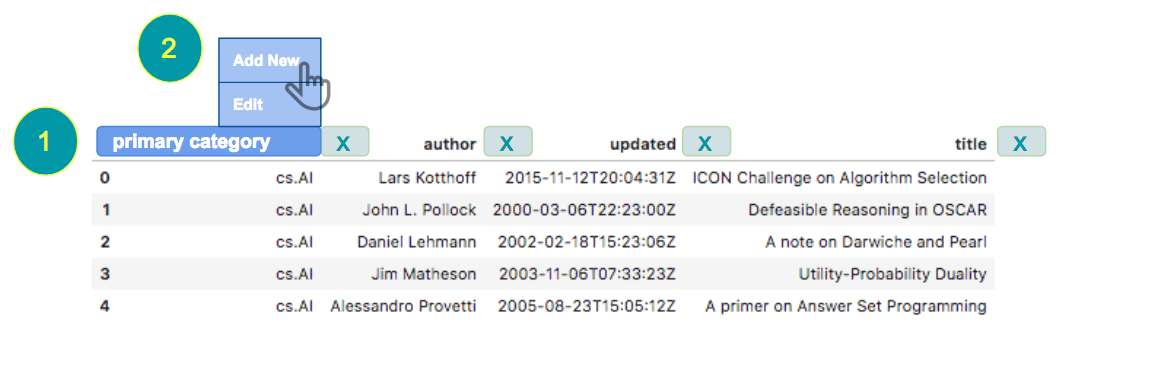
\includegraphics[scale=.3]{figures/m3/wireframe-screen1.png}
\caption{Screen 1: User selects a variable and is given a choice to either edit the existing variable or create a new one based on the selected. Data is retrieved via https://arxiv.org/'s API}
\label{fig::2}
\end{figure}

The user workflow can be described by: 

\begin{itemize}
    \item Select a variable that intended for a transformation. The variable name is highlighted (see Figure~\ref{fig::2}, step 1)
    \item A context menu appears that gives user an option to either \textit{Edit} the existing variable, or \textit{Add New}  (see Figure~\ref{fig::2}, step 2)
    \item Upon selecting to Add a new Variable based on the highlighted field, the user is given a list of Transformations to choose from (See Figure~\ref{fig::3})
    
\begin{figure}[h]
\centering
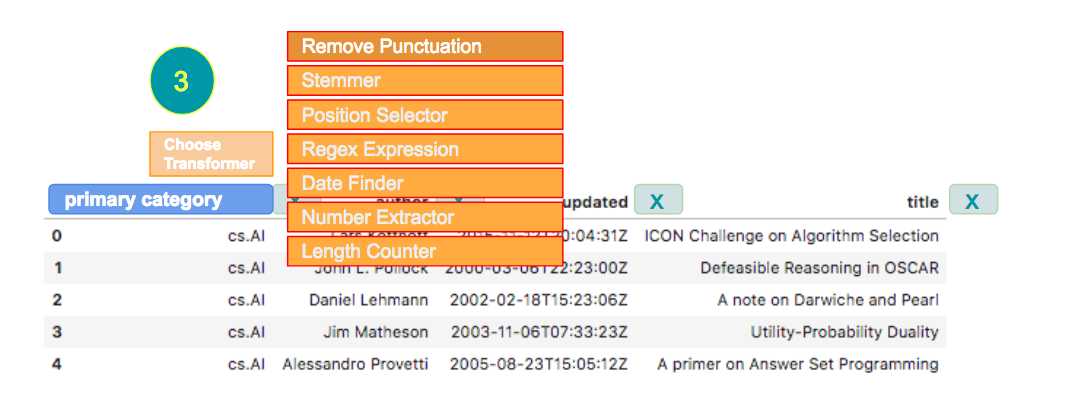
\includegraphics[scale=.3]{figures/m3/wireframe-screen2.png}
\caption{Screen 2: User is given a list of transformations to choose from}
\label{fig::3}
\end{figure}

    \item After the user selected a transformation, a \underline{new block} is created with \underline{a link} to the original variable. A user is prompted to give the new variable a name (see Figure~\ref{fig::4}). The \textit{attached} transformation is kept in the block to remind the user on the selected transformation rule. 
    
    
\begin{figure}[h]
\centering
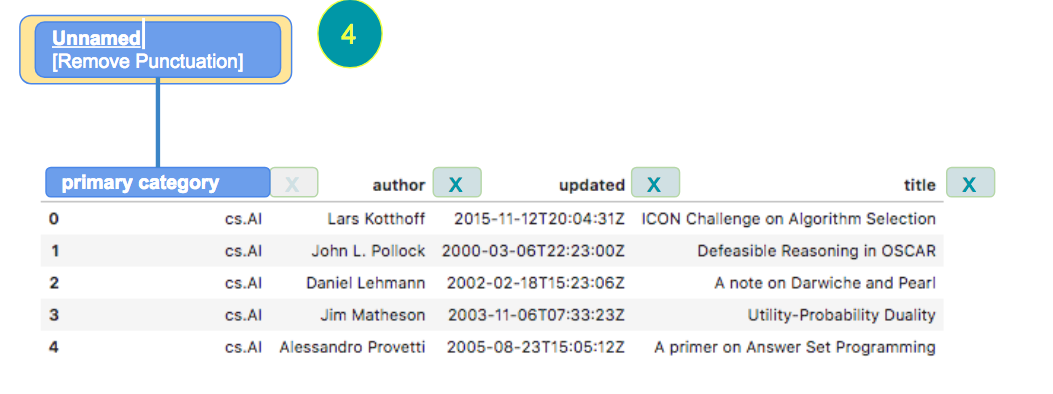
\includegraphics[scale=.3]{figures/m3/wireframe-screen3.png}
\caption{Screen 3: A new block appears that is connected to the selected variable with a cursor prompt to name a new variable}
\label{fig::4}
\end{figure}

    \item Figure~\ref{fig::5} shows a possible view of the outcome of multiple transformations. The information is presented on one screen that given user feedback on the actions taken so far.

\begin{figure}[h]
\centering
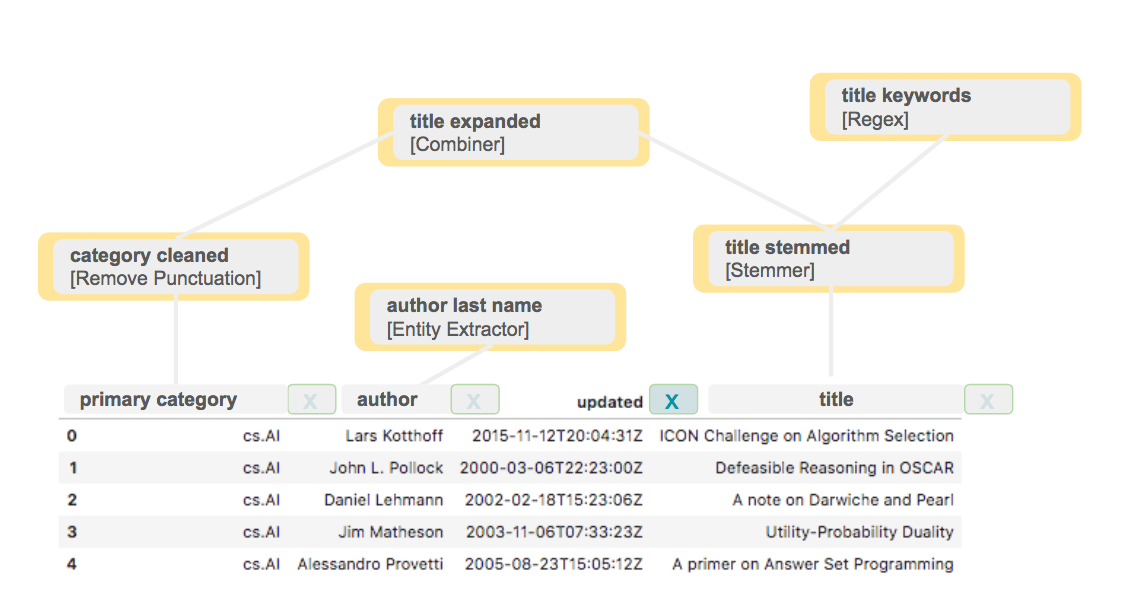
\includegraphics[scale=.3]{figures/m3/wireframe-screen5.png}
\caption{Screen 4: A hypothetical view of the Directed Acyclical Graph (DAG) that is a results of user creating multiple transformations}
\label{fig::5}
\end{figure}

\end{itemize}

\end{document}
